\documentclass[fontset=adobe]{ctexart}

\usepackage{graphicx}
\usepackage{geometry}
\usepackage{hyperref}
\usepackage{hyperxmp}
\usepackage{pdfpages}
\usepackage[bottom]{footmisc}
\usepackage{url}


\newcommand{\artauthor}{陈晟祺;周聿浩}
\newcommand{\arttitle}{FPGA Virtual Console 设计报告}
\newcommand{\artsubject}{基于硬件的 VT220 兼容终端}
\newcommand{\artkeywords}{FPGA;虚拟控制台;Virtual Console}


\hypersetup{pdfauthor=\artauthor,
			pdftitle=\arttitle,
			pdfsubject=\artsubject,
			pdfkeywords=\artkeywords,
			pdfcopyright={Copyright Shengqi Chen & Yuhao zhou 2018. All rights reserved.},
			pdfdate=\today,
			pdfdisplaydoctitle=true,
			pdflang=zh-CN,
			pdfstartview=FitH}

\geometry{
	a4paper,
	left=3.18cm,
	right=3.18cm,
	top=2.54cm,
	bottom=2.54cm
}
\graphicspath{{figures/}}


\begin{document}

\title{{\bf\arttitle\\——\artsubject}}
\author{
计63\hspace{1em}陈晟祺\hspace{1em}2016010981 \\
计64\hspace{1em}周聿浩\hspace{1em}2016011347
}
\date{}
\maketitle

\tableofcontents

\section{项目概述}

\section{架构设计}

\begin{figure}[htbp]
\centerline{
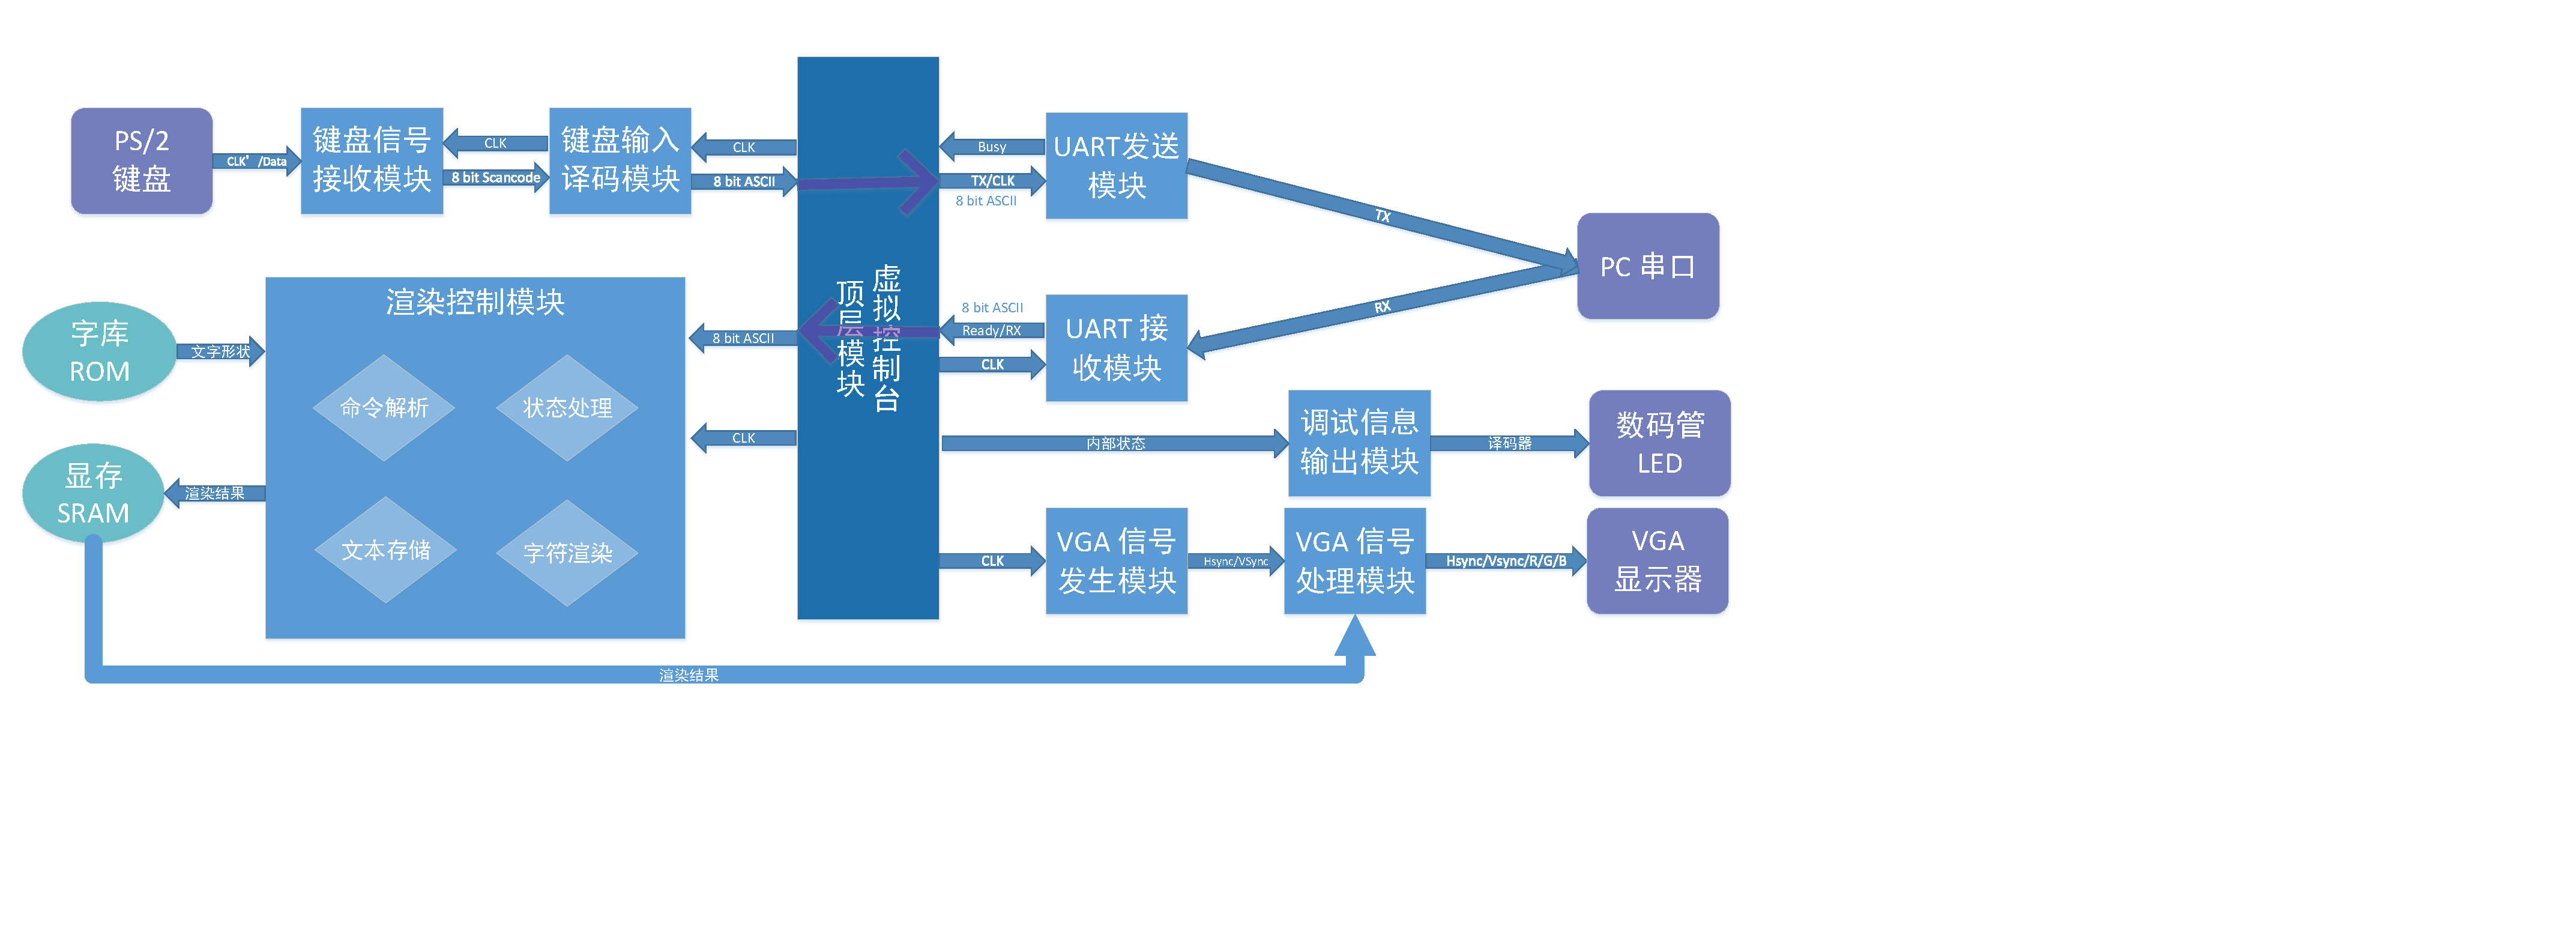
\includegraphics[width=0.95\paperwidth]{architecture_design_visio.pdf}
}
\label{fig:design_architecture}
\caption{项目设计架构}
\end{figure}

\begin{figure}[htbp]
\centerline{
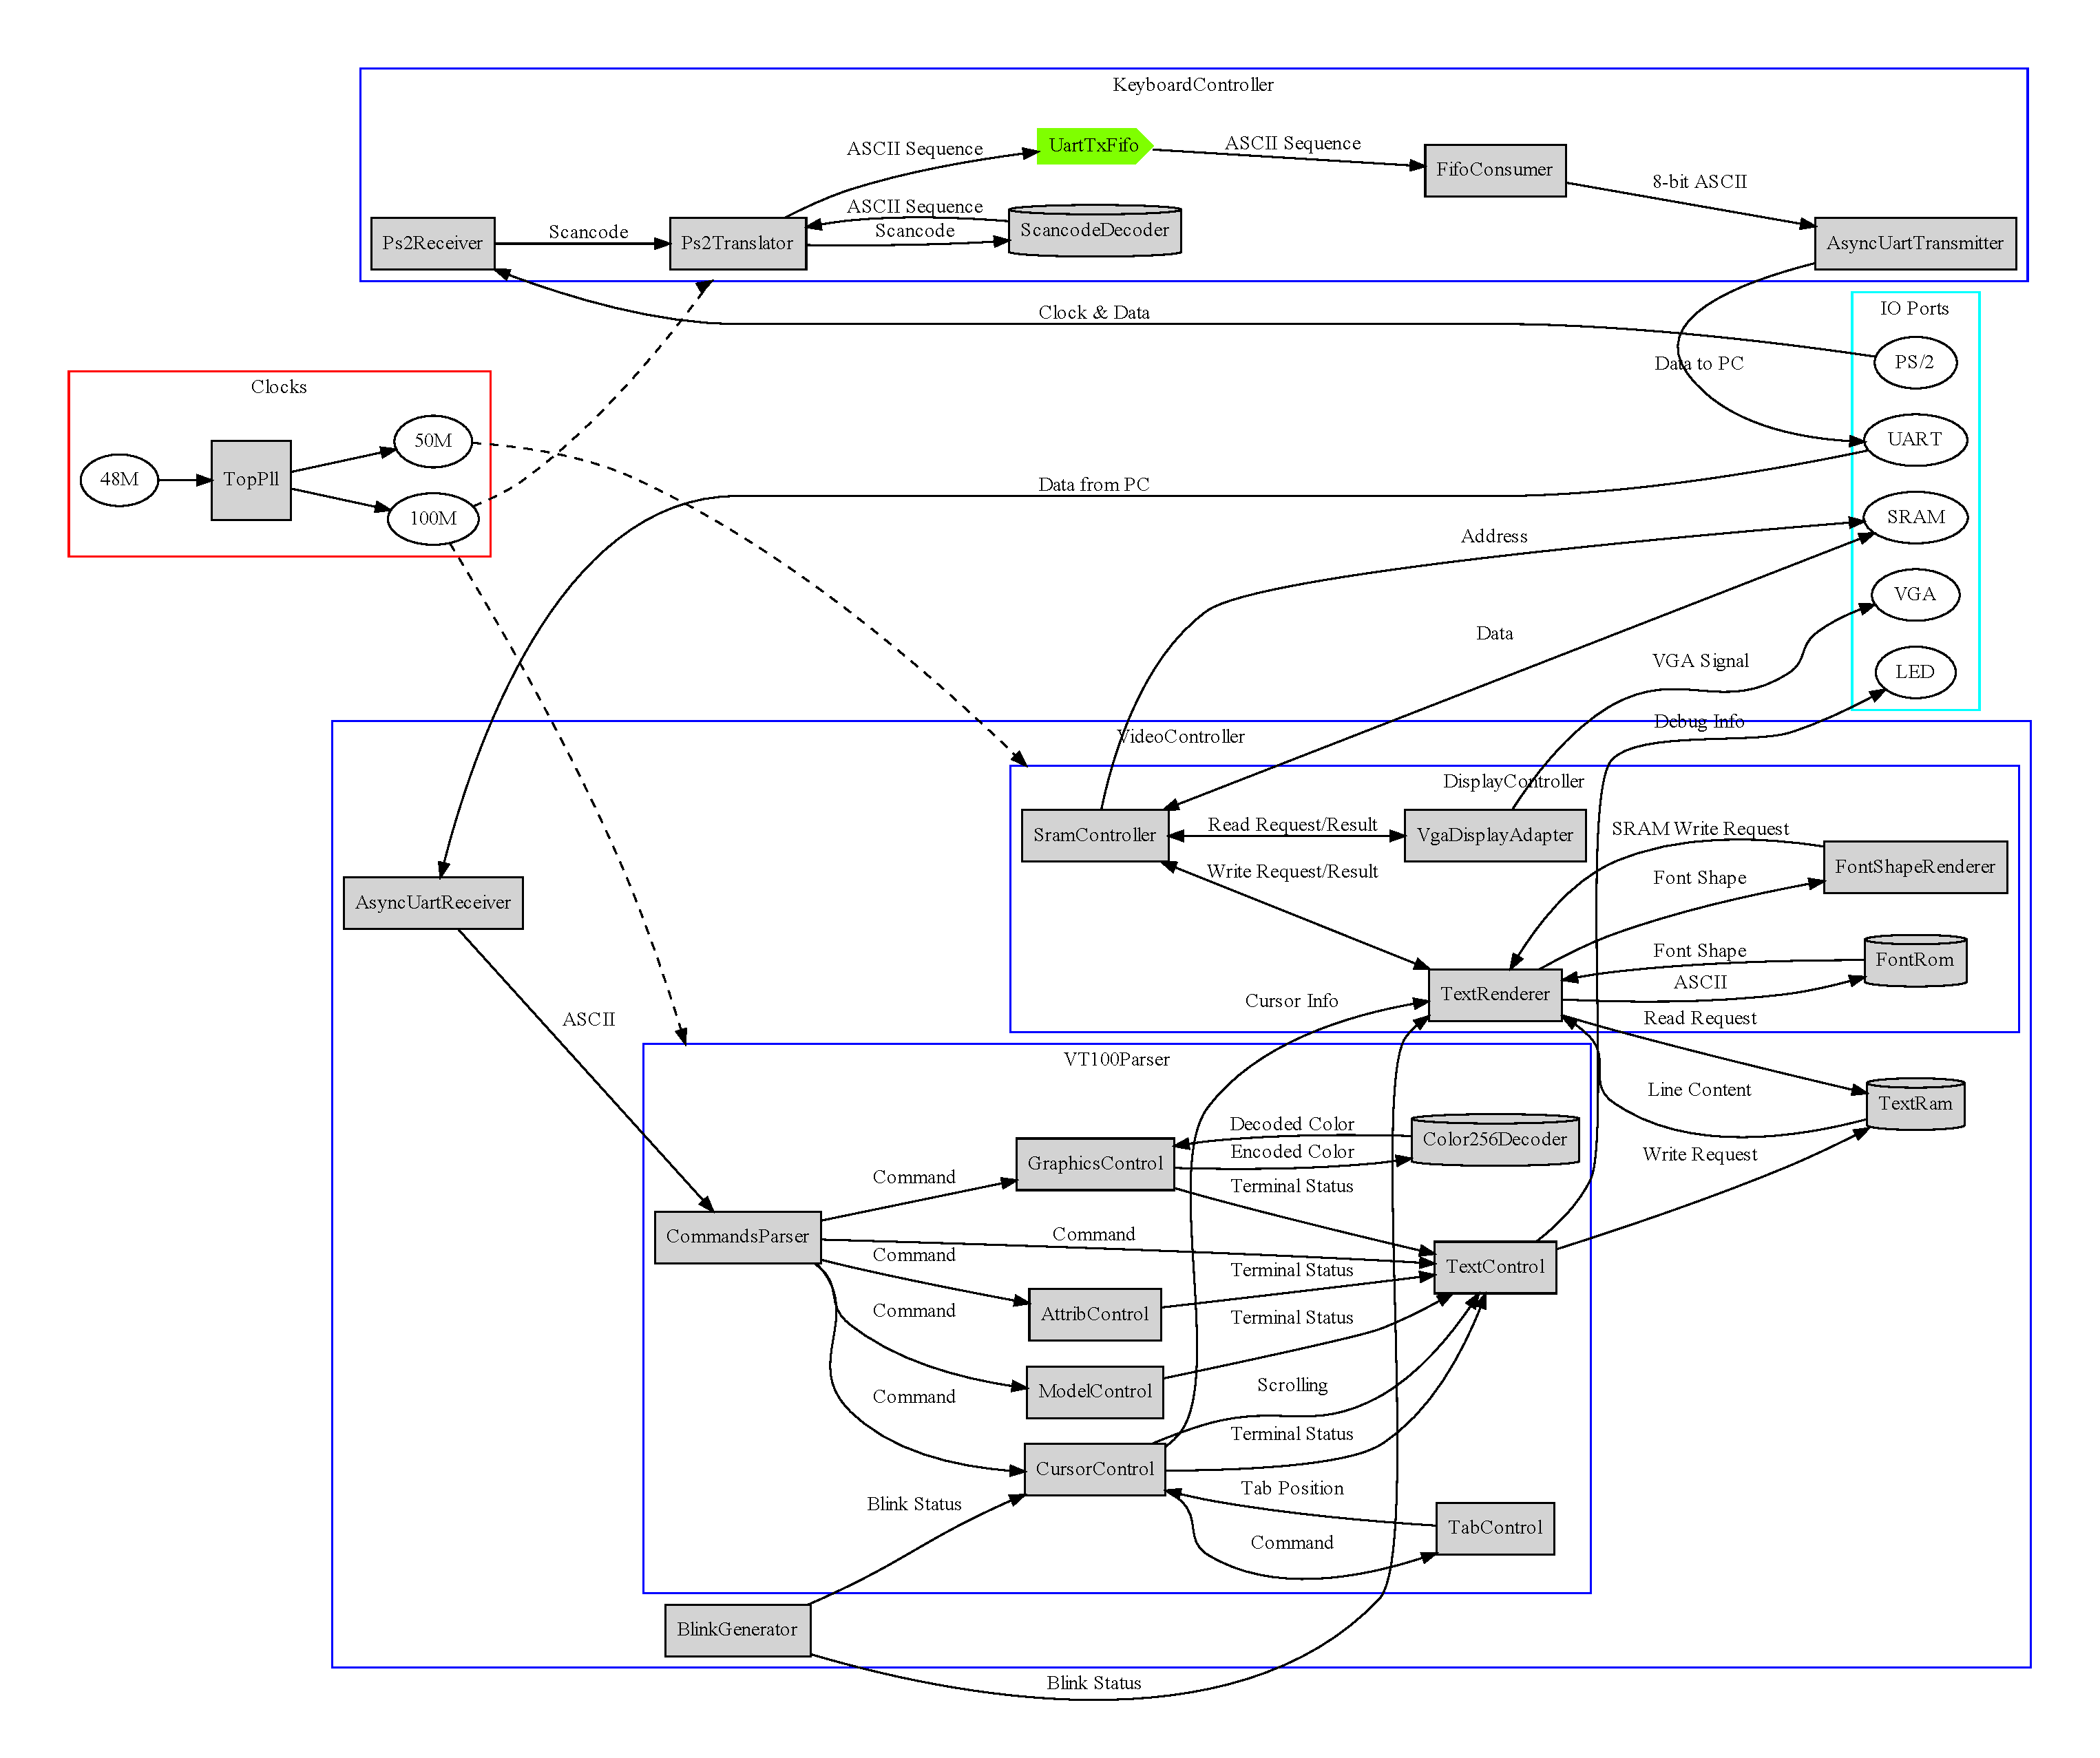
\includegraphics[width=\paperwidth]{architecture_final_dot.pdf}
}
\label{fig:final_architecture}
\caption{项目最终架构}
\end{figure}

\section{模块实现}

\subsection{键盘部分}

\subsection{图形部分}

\section{其他说明}

\end{document}
